\documentclass[12pt]{book}

\usepackage{mathptm,times,color}
\usepackage[pdftex]{graphicx}
\usepackage{multirow}
\usepackage{bezier}
\usepackage{rotating}
\usepackage{longtable}
\usepackage{amsmath}
\usepackage{xfrac}
\usepackage{array}
\usepackage{units}
\usepackage{fix-cm}
\usepackage{makeidx} % Create index at end of document
\usepackage[nottoc,notlof,notlot]{tocbibind} % Put the bibliography and index in the ToC
\usepackage{datetime}
\newdateformat{mydate}{\monthname[\THEMONTH] \THEYEAR}

\usepackage{listings}
\usepackage{textcomp}
\definecolor{lbcolor}{rgb}{0.96,0.96,0.96}
\lstset{
    %backgroundcolor=\color{lbcolor},
    tabsize=4,
    rulecolor=,
    language=Fortran,
        basicstyle=\footnotesize\ttfamily,
        upquote=true,
        aboveskip={\baselineskip},
        belowskip={\baselineskip},
        columns=fixed,
        extendedchars=true,
        breaklines=true,
        breakatwhitespace=true,
        frame=none,
        showtabs=false,
        showspaces=false,
        showstringspaces=false,
        identifierstyle=\ttfamily,
        keywordstyle=\color[rgb]{0,0,0},
        commentstyle=\color[rgb]{0,0,0},
        stringstyle=\color[rgb]{0,0,0},
}

\usepackage{wrapfig}

\newcolumntype{L}[1]{>{\raggedright\let\newline\\\arraybackslash\hspace{0pt}}m{#1}}
\newcolumntype{C}[1]{>{\centering\let\newline\\\arraybackslash\hspace{0pt}}m{#1}}
\newcolumntype{R}[1]{>{\raggedleft\let\newline\\\arraybackslash\hspace{0pt}}m{#1}}

\usepackage{framed}
\newcommand{\graybox}[1]{
\begin{shaded}#1\end{shaded}
}

\renewcommand{\bibname}{References}

% dummy change to force revision update

%\usepackage{eso-pic}
%\usepackage{graphicx}
%\usepackage{color}
%\usepackage{type1cm}


%\makeatletter
%   \AddToShipoutPicture{%
%     \setlength{\@tempdimb}{.5\paperwidth}%
%    \setlength{\@tempdimc}{.5\paperheight}%
%   \setlength{\unitlength}{1pt}%
%  \put(\strip@pt\@tempdimb,\strip@pt\@tempdimc){%
%     \makebox(0,0){\rotatebox{45}{\textcolor[gray]{0.75}{\fontsize{8cm}{8cm}\selectfont{DRAFT}}}}}}
%\makeatother

\definecolor{linknavy}{rgb}{0,0,0.50196}
\definecolor{linkred}{rgb}{1,0,0}
\definecolor{linkblue}{rgb}{0,0,1}
\definecolor{shadecolor}{rgb}{0.9,0.9,0.9}

\usepackage[pdftex,
        colorlinks=true,
        urlcolor=linkblue,     % \href{...}{...} external (URL)
        citecolor=linkred,     % citation number colors
        linkcolor=linknavy,    % \ref{...} and \pageref{...}
        pdfproducer={pdflatex},
        pagebackref,
        pdfpagemode=UseNone,
        bookmarksopen=true,
        plainpages=false,
        verbose]{hyperref}

% CFAST Version String
\newcommand{\cfastversion}{7.0.0}

% commands to use for "official" cover and title pages
% see smokeview verification guide to see how they are used

\newcommand{\logosigs}{
\begin{minipage}[b]{6.5in}
\flushright{
\includegraphics[height=1.05in]{FIGURES/nistident}}
\end{minipage}
}

\newcommand{\titlesigs}
{
\small
\begin{flushright}
U.S. Department of Commerce \\
{\em Penny Pritzker, Secretary} \\
\hspace{1in} \\
National Institute of Standards and Technology \\
{\em Willie May, Acting Under Secretary of Commerce for Standards and Technology and Acting Director}
\end{flushright}
}

\newcommand{\headerA}[1]{
\begin{flushright}
\fontsize{20}{24}\selectfont
\bf{NIST Technical Note #1}
\end{flushright}
}


\newcommand{\headerB}[1]{
\begin{flushright}
\fontsize{28}{33.6}\selectfont
\bf{#1}
\end{flushright}
}

\newcommand{\headerC}[1]{
\vspace{.15in}
\begin{flushright}
\fontsize{12}{14}\selectfont
#1
\end{flushright}
}

\newcommand{\headerD}[1]{
\begin{flushright}
\fontsize{12}{14}\selectfont
This publication is available free of charge from: \\
http://dx.doi.org/10.6028/NIST.TN.#1
\end{flushright}
}



\setlength{\textwidth}{6.5in}
\setlength{\textheight}{9.0in}
\setlength{\topmargin}{0.in}
\setlength{\headheight}{0.in}
\setlength{\headsep}{0.in}
\setlength{\parindent}{0.25in}
\setlength{\oddsidemargin}{0.0in}
\setlength{\evensidemargin}{0.0in}


\newcommand{\brackets}[1]{ { \left( {#1} \right) } }
\newcommand{\dbydt}[1]{\frac{d {#1}}{dt}}
\newcommand{\superscript}[1]{\ensuremath{^{\textnormal{\scriptsize \hbox{#1}}}}}
\newcommand{\subscript}[1]{\ensuremath{_{\textnormal{\scriptsize \hbox{#1}}}}}

\newcommand{\trho}{\tilde{\rho}}
\newcommand{\dph}{{\delta\phi}}
\newcommand{\dth}{{\delta\theta}}
\newcommand{\tp}{\tilde{p}}
\newcommand{\dQ}{\dot{Q}}
\newcommand{\dQc}{\dot{Q}_{\rm c}}
\newcommand{\dQr}{\dot{Q}_{\rm r}}
\newcommand{\Dh}{\Delta h}
\newcommand{\DhO}{\Delta h_\OTWO}
\newcommand{\Tp}{T_{\rm p}}
\newcommand{\Tu}{T_{\rm u}}
\newcommand{\Tl}{T_{\rm l}}
\newcommand{\Ts}{T_{\rm s}}
\newcommand{\Tg}{T_{\rm g}}
\newcommand{\TL}{T_{\rm L}}
\newcommand{\Vu}{V_{\rm u}}
\newcommand{\Vl}{V_{\rm l}}
\newcommand{\doh}{\dot{h}}
\newcommand{\dhl}{\dot{h}_{\rm l}}
\newcommand{\dhu}{\dot{h}_{\rm u}}
\newcommand{\dmal}{\dot{m}_{\rm l}}
\newcommand{\dmau}{\dot{m}_{\rm u}}
\newcommand{\dq}{\dot{q}}
\newcommand{\dqc}{\dot{q}_{\rm c}}
\newcommand{\dqr}{\dot{q}_{\rm r}}
\newcommand{\dm}{\dot{m}}
\newcommand{\dme}{\dot{m}_{\rm e}}
\newcommand{\dmp}{\dot{m}_{\rm p}}
\newcommand{\dml}{\dot{m}_{\rm l}}
\newcommand{\dmu}{\dot{m}_{\rm u}}
\newcommand{\dmf}{\dot{m}_{\rm f}}

\newcommand{\be}{\begin{equation}}
\newcommand{\ee}{\end{equation}}

\newcommand{\RE}{\hbox{Re}}
\newcommand{\LE}{\hbox{Le}}
\newcommand{\PR}{\hbox{Pr}}
\newcommand{\PE}{\hbox{Pe}}
\newcommand{\NU}{\hbox{Nu}}
\newcommand{\SC}{\hbox{Sc}}
\newcommand{\SH}{\hbox{Sh}}
\newcommand{\WE}{\hbox{We}}

\newcommand{\COTWO}{{\tiny \hbox{CO}_2}}
\newcommand{\OTWO}{{\tiny \hbox{O}_2}}
\newcommand{\CO}{{\tiny \hbox{CO}}}
\newcommand{\HTWOO}{{\tiny \hbox{H}_2\hbox{O}}}
\newcommand{\NTWO}{{\tiny \hbox{N}_2}}
\newcommand{\F}{{\tiny \hbox{F}}}
\newcommand{\So}{{\tiny \hbox{S}}}
\newcommand{\M}{{\tiny \hbox{M}}}
\newcommand{\HCN}{{\tiny \hbox{HCN}}}
\newcommand{\HCl}{{\tiny \hbox{HCl}}}
\newcommand{\Hy}{{\tiny \hbox{H}}}
\newcommand{\C}{{\tiny \hbox{C}}}
\newcommand{\N}{{\tiny \hbox{N}}}
\newcommand{\Oh}{{\tiny \hbox{O}}}
\newcommand{\Cl}{{\tiny \hbox{Cl}}}

\newcommand{\asqh}{$A_T/A\sqrt{h}$}
\newcommand{\degc}{$^{\circ}$C }
\newcommand{\degf}{$^{\circ}$F }

\newcommand{\dx}{\delta x}
\newcommand{\dy}{\delta y}
\newcommand{\dz}{\delta z}
\newcommand{\dt}{\delta t}

\newcommand{\ha}{\frac{1}{2}}
\newcommand{\ft}{\frac{4}{3}}
\newcommand{\ot}{\frac{1}{3}}
\newcommand{\fofi}{\frac{4}{5}}
\newcommand{\of}{\frac{1}{4}}
\newcommand{\twth}{\frac{2}{3}}


\newcommand{\rb}[1]{\raisebox{1.5ex}[0pt]{#1}}

\newcommand{\erf}{\hbox{erf}}



\begin{document}

\bibliographystyle{unsrt}

\frontmatter

\pagestyle{empty}


\begin{minipage}[t][9in][s]{6.5in}

\headerA{XXXX\\}

\headerB{
CFAST -- Consolidated Fire \\
 and Smoke Transport \\
 (Version 7) \\
 Volume 4: Configuration Management \\
}

\headerC{
   Richard D. Peacock \\
}

\vfill

\headerD{XXXXv4}

\vfill

\logosigs

\end{minipage}

\newpage

\hspace{5in}

\newpage

\begin{minipage}[t][9in][s]{6.5in}

\headerA{XXXX\\}

\headerB{
CFAST -- Consolidated Fire \\
 And Smoke Transport \\
 (Version 7) \\
 Volume 4: Configuration Management \\
}

\headerC{
   Richard D. Peacock \\
}

\headerD{XXXXv4}

\headerC{
\flushright{\mydate\today\\
CFAST Version \cfastversion \\
\emph{SVN Repository}~$Revision$}}
% dummy comment to force svn change - Mon Jan  5 21:57:14 EST 2015

\vfill

\flushright{
\includegraphics[width=1.2in]{FIGURES/doc} }

\titlesigs

\end{minipage}


\newpage

\frontmatter

\pagestyle{plain}
\setcounter{page}{3}


\chapter{Preface}

The purpose of this document is to describe the policies and procedures for developing and maintaining CFAST. Such a document is commonly referred to as a {\em Configuration Management Plan}. Description of the theoretical basis of the model, instructions for its are contained in a separate user's guide, and model assessment information is contained in a separate verification and validation guide.

\chapter{Disclaimer}

The US Department of Commerce makes no warranty, expressed or implied, to users of CFAST, and accepts no responsibility for its use. Users of CFAST assume sole responsibility under Federal law for determining the appropriateness of its use in any particular application; for any conclusions drawn from the results of its use; and for any actions taken or not taken as a result of analysis performed using these tools.

Users are warned that CFAST is intended for use only by those competent in the fields of fluid dynamics, thermodynamics, heat transfer, combustion, and fire science, and is intended only to supplement the informed judgment of the qualified user. The software package is a computer model that may or may not have predictive capability when applied to a specific set of factual circumstances. Lack of accurate predictions by the model could lead to erroneous conclusions with regard to fire safety. All results should be evaluated by an informed user.

Throughout this document, the mention of computer hardware or commercial software does not constitute endorsement by NIST, nor does it indicate that the products are necessarily those best suited for the intended purpose.




\chapter{Acknowledgments}

\label{acksection}

CFAST was originally developed by Walter Jones, formerly of NIST.

Continuing support for CFAST is via internal funding at NIST. In addition, support is provided by other agencies of the U.S. Federal Government, most notably the Nuclear Regulatory Commission (NRC) and the Department of Energy (DOE). The NRC Office of Research has funded key validation experiments, the preparation of the CFAST manuals, and the continuing development of sub-models that are of importance in the area of nuclear power plant safety. Special thanks to Mark Salley and David Stroup for their support. Support to refine the software development and quality assurance process for CFAST has been provided by the U.S. Department of Energy. The assistance of Subir Sen and Debra Sparkman is gratefully acknowledged.

The idea for this Guide originated with Jason Floyd, a co-developer of FDS and practicing engineer at Jensen Hughes. He readily saw the need for a clear description of the process of developing and maintaining FDS and Smokeview. This guide adapts the FDS process for the CFAST model.  Bryan Klein, currently with Thunderhead Engineering, Inc., and Kristopher Overholt, currently with Continuum Analytics instituted a number of the internet tools that are described in the Guide, including the source code repository, issue tracking system, and discussion group sites.


\tableofcontents

\listoffigures


\mainmatter

\chapter{Overview}

CFAST is a two-zone fire model that predicts the thermal environment caused by a fire within a compartmented structure. Each compartment is divided into an upper and lower gas layer. The fire drives combustion products from the lower to the upper layer via the plume. The temperature within each layer is uniform, and its evolution in time is described by a set of ordinary differential equations derived from the fundamental laws of mass and energy conservation. The transport of smoke and heat from zone to zone is dictated by empirical correlations. Because the governing equations are relatively simple, CFAST simulations typically require a few tens of seconds of CPU time on typical personal computers.

The purpose of this document is to describe the policies and procedures for developing and maintaining CFAST. Such a document is commonly referred to as a {\em Configuration Management Plan}, known through the rest of this document as ``the Plan.'' This document will be updated as the necessity arises and will establish and provide the basis for a uniform and concise standard of practice for CFAST development. It is based in part on IEEE Standard 828~\cite{IEEE-828} and ASTM~E1355~\cite{ASTM:E1355}.

The volumes that make up the CFAST Technical Reference Guide are based in part on ASTM E 1355, {\em Standard Guide for Evaluating the Predictive Capability of Deterministic Fire Models}~\cite{ASTM:E1355}. ASTM~E~1355 outlines the process of assessing the accuracy of a fire model. Volumes~1 through 3 are the result of this evaluation process. The main purpose of the present volume is to describe the process by which the model software is developed and maintained. A model such as CFAST cannot remain static. As progress is made in fire science, the model needs to be updated and improved, but still shown to reliably predict the kinds of
phenomena for which it was originally designed.

This document describes the processes used during the development and deployment of the Consolidated Fire and Smoke Transport model (CFAST).  This software quality assurance (SQA) plan is intended to guide the planning for modifications to the model, provide required reviews for both software and associated documentation of the model, define testing to be conducted prior to the release of an updated model, describe problem reporting and resolution procedures, and ensure all records, source code, and released software is kept available for the life of the code.  While this memorandum and many of our practices follow the Institute of Electrical and Electronics Engineers (IEEE) standard for software quality assurance, IEEE 730-2002 \cite{IEEE:730}, other standards have been followed as well.  Most notably, ASTM 1355-05, ``Standard Guide for Evaluating the Predictive Capability of Deterministic Fire Models'' \cite{ASTM:E1355} has been used extensively to guide the documentation, verification, and validation of the model.

CFAST is intended for use only by those competent in the field of fire safety and is intended only to supplement the informed judgment of the qualified user. The software package is a computer model which has limitations based on the way it is used, and the data used for calculations. All results should be evaluated by a qualified user.

The SQA process and requirements outlined in this document apply specifically to the CFAST and is focused on ensuring the quality of the numerical predictions of the model.  The user interface that may be used to develop input for the model is included in this process to insure that changes to the model are reflected in the user interface and in the data files created by the user interface for use by the model.  Of course, users must ensure that the input files developed for the simulations accurately reflect the desired model inputs, whether developed using the supplied user interface, another third-party interface, or manually input with a spreadsheet or text editor program.  Documentation of these inputs is included as part of the model documentation outlined below.

Documentation and configuration management for its companion visualization program Smokeview, is documentation for FDS and Smokeview.

\chapter{Relevant Publications}

To accompany the model and simplify its use, NIST has developed a Technical Reference Guide \cite{CFAST_Tech_Guide_7} and a User's Guide \cite{CFAST_Users_Guide_7} a Validation Guide \cite{CFAST_Valid_Guide_7}, and this Configuration Management Guide..  The Technical Reference Guide describes the underlying physical principles and summarizes sensitivity analysis, model validation, and model limitations consistent with ASTM E 1355 \cite{ASTM:E1355}.  The User's Guide describes how to use the model.  The Validation Guide documents sensitivity analyses, model verification, model validation, and model limitations consistent with ASTM~E1355~\cite{ASTM:E1355}.

The U.S. Nuclear Regulatory Commission has published a verification and validation study of five selected fire models commonly used in support of risk-informed and performance-based fire protection at nuclear power plants \cite{NRCNUREG1824}. In addition to an extensive study of the CFAST model, the report compares the output of several other models ranging from simple hand calculations to more complex CFD codes such as the Fire Dynamics Simulator (FDS) developed by NIST.

While this document and many of our practices make extensive use of ASTM 1355, ``Standard Guide for Evaluating the Predictive Capability of Deterministic Fire Models'' \cite{ASTM:E1355} to guide the documentation, verification, and validation of the model, other standards have been followed as well.  Most notably, our software quality assurance processes were guided by the IEEE standard for software quality assurance, IEEE 730-2002 \cite{IEEE:730}.

In addition, numerous related documents available at http://cfast.nist.gov provide a wealth of information concerning including earlier versions of the model and its user interface. Software quality assurance (SQA) plan is intended to guide the planning for modifications to the model, provide required reviews for both software and associated documentation of the model, define testing to be conducted prior to the release of an updated model, describe problem reporting and resolution procedures, and ensure all records, source code, and ensure released software is kept available for the life of the code.

\chapter{Model Identification and Control}

CFAST is developed and maintained by the Engineering Laboratory (EL) at the National Institute of Standards and Technology (NIST). Like all projects at NIST, a designated project leader is responsible for directing and prioritizing model development, error correction, and preparation of documentation for the model development.  The organization chart in Figure \ref{figOrgChart} provides a graphical representation of the software quality organization structure for CFAST

\begin{figure}
\begin{center}
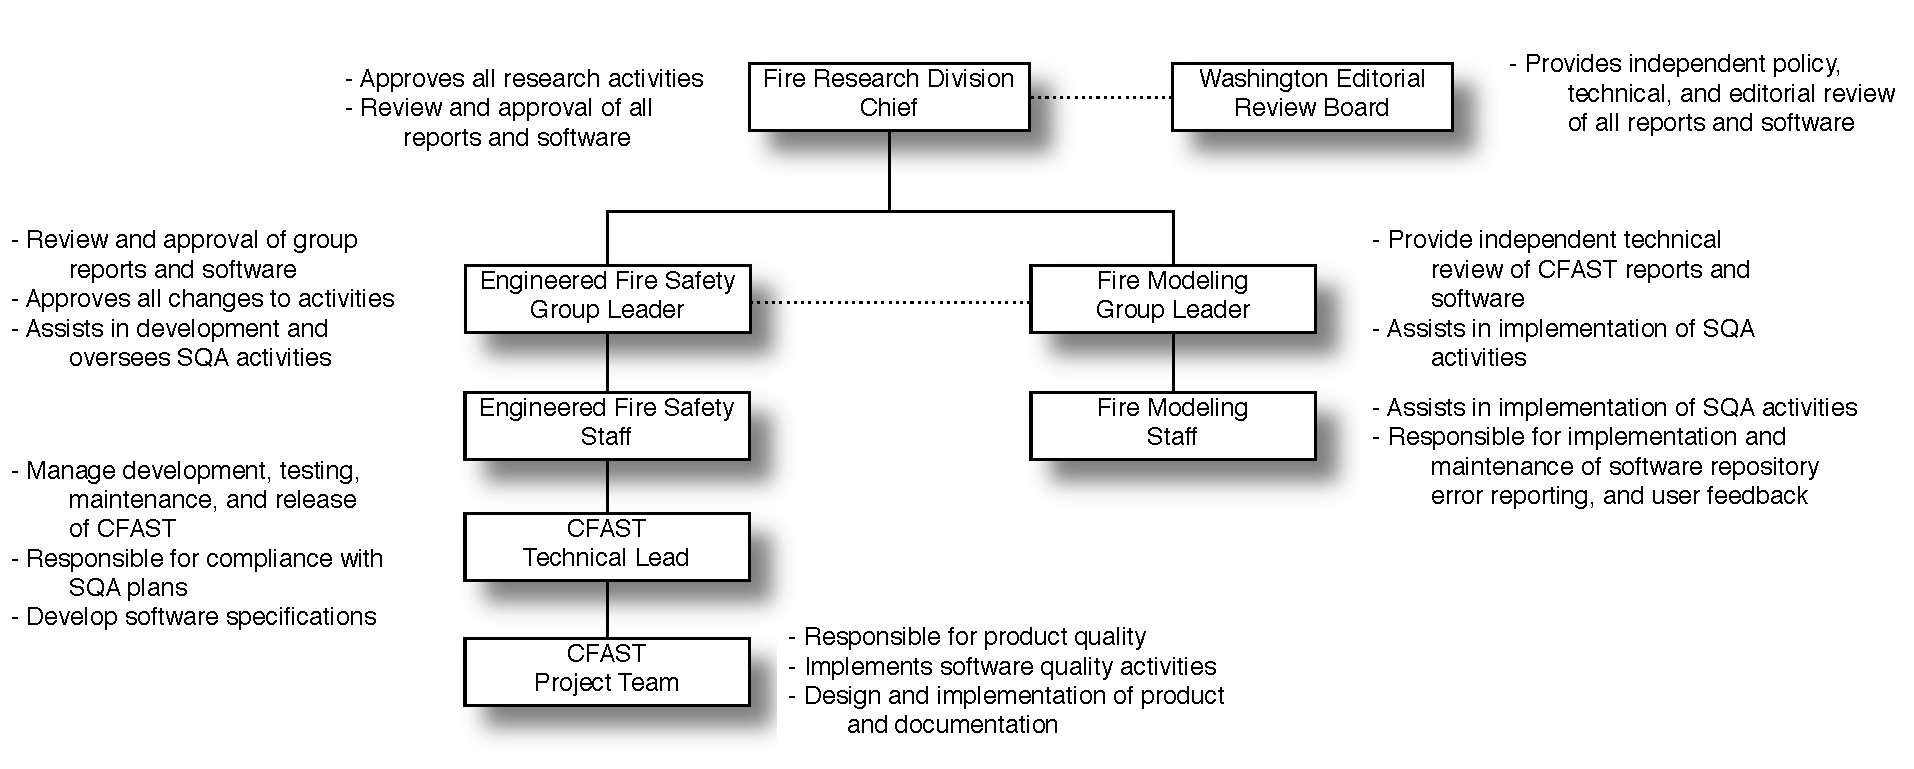
\includegraphics[width=6.5in]{FIGURES/OrgChart.pdf}\\
\end{center}
\caption{CFAST SQA Organization Structure.}
 \label{figOrgChart}
\end{figure}

Review and approval of software and documentation is part of the standard review process for any report or other product developed by NIST. A minimum of five reviews are required prior to release of reports or software, including two independent technical peer reviews, two technical and management reviews at the technical workgroup and division level, and a policy review at the NIST-wide level.  This review is documented and recorded on the NIST standard form NIST 114 along with official approval notification provided to the primary author of the product.

CFAST is distributed exclusively through a NIST website dedicated to the CFAST model (http://cfast.nist.gov).  Content of the website is the responsibility of the CFAST project leader and the NIST webmaster. Additions and changes to the website are made only with the approval of the CFAST project leader after any required NIST reviews.

Document identification and control consists of placing all project files in a central location and maintaining a record of changes to those files. The central location is known as the {\em Repository}.

\section{Project Repository}

CFAST and Smokeview make use of Google Code Project Hosting, a free service offered by Google to support software development for open source applications.  Google Code uses the Subversion (SVN) revision management system. Under this system a centralized repository containing all project files resides on a Google Code server. Subversion uses a single integer that identifies the version of the entire repository rather than a specific file (i.e., anytime a change is made to the repository all files are incremented in version number).  A record of version number when a specific file was last changed is maintained. As an open source program, any individual can obtain a copy of the repository or retrieve specific versions of the repository.  Only Team Members described in the previous chapter can commit changes to the repository.

The current location of the CFAST repository is \href{http://cfast.googlecode.com/svn/trunk/}{\textct{http://cfast.googlecode.com/svn/trunk/}}. The repository contains the following files:
\begin{enumerate}
\item Compiled CFAST and Smokeview executables
\item CFAST source code files
\item CFAST documentation
\item Input files for software testing, verification testing, and validation testing
\item Experimental data files used for validation testing
\item Scripts and post-processing utilities used for software testing
\item Web pages and wikis containing notes and other information
\end{enumerate}
In the event of an unexpected change to the Google Code service and/or the CFAST repository, each member of the development team, plus interested third parties, has a copy of the repository on their local computer. At NIST, the staff computers are regularly backed up as well. Thus, there is very little chance that the project repository will be lost. If need be, the files could be moved to another open source software development site, such as SourceForge. It is expected that if Google decides to end its support for Google Code, it will provide its users with the full history of the project.

\section{Version Identification}

At the start of a simulation, CFAST writes header information to the Smokeview output file, CFAST output file, and the CFAST log file.  This header information contains the version of CFAST used to perform that simulation. While each release is tagged with a specific version number (e.g., 7.0.0), there may be many commits of source code, documentation, or other files to the SVN repository before a new version is released with an incremented version number.  Thus, if a developer or a user who performs their own compilation between baseline releases discovers an error, the version number written to the output files may not be sufficient to identify the specific set of source code files used.  Rather, one would need to know the SVN revision number of the most recently committed source file. This is accomplished by using source file tagging. In each source file, a series of character parameter strings are defined. For example, near the bottom of the source file {\ct cfast.f90} are lines of the form:
\begin{lstlisting}
character(255), parameter :: mainrev='$Revision: 2137 $'
character(255), parameter :: maindate='$Date: 2015-04-14 13:45:07 -0400 (Tue, 14 Apr 2015) $'
\end{lstlisting}
The lines contain the name of the source file, the version of the file (this reflects only the source file version and not the overall release version number), the date and time of the file version, and the person who checked the file into the repository. Upon compiling, these strings will be stored in the executable file.  The user can search the executable file for strings beginning with \textct{\$Id:}, which results in a list of all source files compiled and their version. Within the SVN archive, any specific version of a source file can be extracted and differences between versions can be determined.

Within the source code a series of subroutines were created, one per source file, which parses the \textct{\$Id:} in each file and extracts from it the SVN revision number.  Each of these subroutines is called at the start of an CFAST run and the largest (and hence most recent) revision number is determined.  This number is written along with the CFAST version number to the output header information.  A user can now identify specifically the source code used for a particular compilation of CFAST when reporting an error.


\chapter{SQA Documentation}

The released version of CFAST is documented by three primary publications, the Technical Reference Guide\cite{CFAST_Tech_Guide_7}, the User's Guide \cite{CFAST_Users_Guide_7}, and this Software and Model Evaluation Guide. The documents apply to the newest version of the model available on the NIST website. The Technical Reference Guide describes the underlying physical principles, provides a review of model verification and validation efforts by NIST and others, and describes the limitations of the model.  The User's Guide describes how to use the model, includes a detailed description of the model inputs and outputs, and provides a process to ensure the correct installation of the model. There are also documents archived on the website that are applicable to older versions of both the model and user interface.

\section{Development Process}

Changes are made to the CFAST source code daily, and tracked via revision control software. However, these daily changes do not constitute a change to the version number. After the developers determine that enough changes have been made to the source, they release a new minor upgrade, 6.2.1 to 6.2.2, for example. This happens every few weeks. A change from 6.2 to 6.3 might happen only once a year, when significant improvements have been made to the model physics or numerics.

There is no formal process by which CFAST is updated. Each developer works on various routines, and makes changes as warranted. Minor bugs are fixed without any communication (the developers are in different locations), but more significant changes are discussed via email or telephone calls. A suite of simple verification calculations (included in this document) are run each night to ensure that the daily bug fixes have not altered any of the important algorithms. A suite of validation calculations (also included here) are run each night. Significant changes to CFAST are made based on the following criteria, in no particular order:
\begin{description}
\item[Better Physics:] The goal of any model is to be {\em predictive}, but it also must be reliable. CFAST is a blend of empirical and deterministic sub-models, chosen based on their robustness, consistency, and reliability. Any new sub-model must demonstrate that it is of comparable or superior accuracy to its empirical counterpart.
\item[Simpler Algorithm:] If a new algorithm does what the old one did using fewer lines of code, it is almost always accepted, so long as it does not decrease functionality or accuracy.
\item[Increased or Comparable Accuracy:] The validation experiments that are part of this guide serve as the metric for new routines. It is not enough for a new algorithm to perform well in a few cases. It must show clear improvement across the entire suite of experiments. If the accuracy is only comparable to the previous version, then some other criteria must be satisfied.
\item[Acceptance by the Fire Protection Community:] Especially in regard to fire-specific devices, like sprinklers and smoke detectors, the algorithms in CFAST often are based on their acceptance among the practicing engineers.
\end{description}

\subsection{Creating a Change Request}

Change requests are submitted using the CFAST Issue Tracker.  The Issue Tracker is an online service provided by Google Code Project Hosting. To submit a new issue to the tracker or to provide follow up comments, the user must sign in using his or her Google account credentials. A change request is initiated by opening a new issue.  The issue report contains the baseline identification (version number, compile date, and SVN revision number), operating system, and a description of the defect or enhancement request.  Input files or other supporting documentation can be attached.
\begin{figure}[ht!]
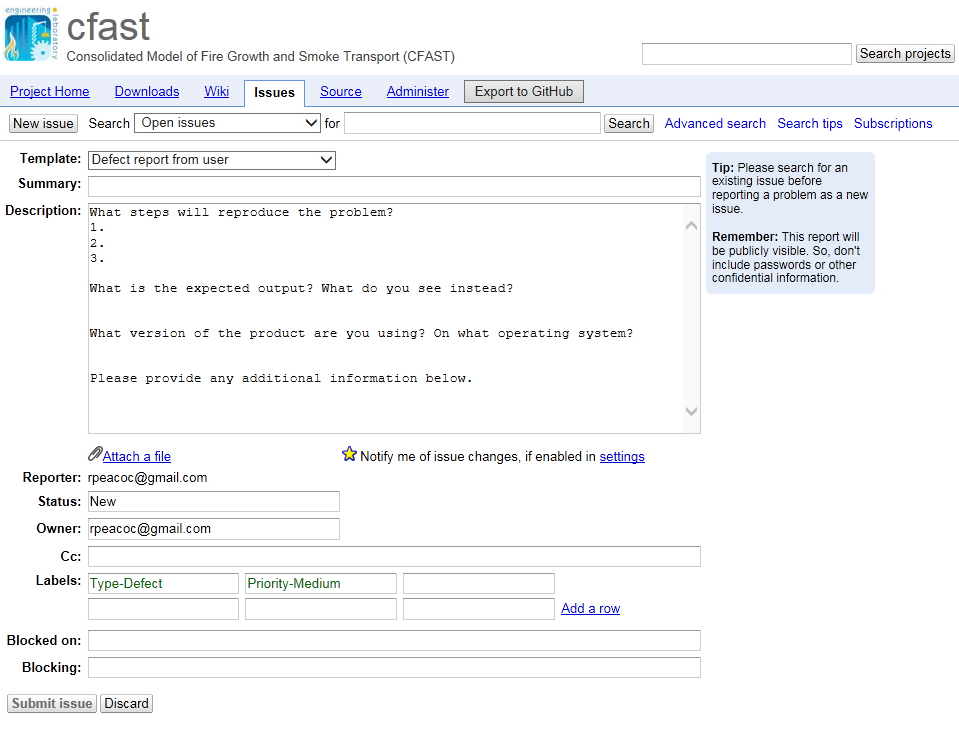
\includegraphics[width=\textwidth]{FIGURES/NewIssue}
\caption{Screenshot of issue tracker reporting form}
\label{fig:issueform}
\end{figure}
If the issue is opened by a user, it will be given a status of \textct{New} until it is reviewed by a developer. This typically takes a few minutes to a few hours, depending on the time of day the issue is reported. If the issue is opened by a developer, the developer can immediately assign a status and an owner.

\subsection{Processing a Change Request}

A change request may be evaluated by any member of the development team. If the request duplicates an existing request, then the issue status is changed to \textct{Duplicate} and the
requestor is sent the issue number of the existing request.

If the request is for an enhancement to CFAST, then the issue type is changed to \textct{Type-Enhancement} and the component type is declared. The request is evaluated for suitability.  If it is a valid enhancement request, then the status is changed to \textct{Accepted}.  If the request is not to be addressed under the next baseline, then the status will be changed to \textct{OnHold}.  If the request is denied, then the status is changed to \textct{WontFix}.  An accepted request will be assigned to a developer.

If the request is identifying a defect in CFAST, then the issue type is changed to \textct{Type-Defect} and the component type is declared.  The defect is evaluated for validity.  If insufficient information has been provided in the request, then the status is changed to \textct{MoreInfo} and a description of the additional information required is sent to the requestor.  If the defect is due to user error or is the intended function of CFAST, then the status is changed to \textct{Invalid}.  If the defect is valid, then the request reviewer will change the status to \textct{Accepted} and assign the request to a developer.

Once a change request has be addressed by a developer and changes submitted to the repository, the request status is changed to \textct{Fixed}.  Once either the requestor or another developer has verified that the changes address the original request, then the status is changed to \textct{Verified}.


\subsection{Committing Changes}

Once a developer has addressed a change request, the modified files are committed to the SVN repository.  A description of the changes will be added to the SVN change log.  This description first identifies the primary component being changed (for example: CFAST Source or CFAST Documentation).  This component identification will be followed by a brief summary of the changes made.

Changes to the CFAST source code and supporting documentation are reviewed by other members of the team. There is no formal system with which changes are reviewed because the frequency of changes makes it impractical. As a general rule, all team members watch for unintentional commits of copyrighted material or algorithms, and also proprietary data or case studies collected from an end user. CFAST itself does not include copyrighted or proprietary data, but occasionally this kind of information is submitted by an end user who has submitted a bug report.

\subsection{Change Verification}

Once a change has been committed and the issue tracker updated to reflect that the issue has been \textct{Fixed}, the changes will be verified.  Verification can be done by either the requester of the change or by another developer.  Once the changes have been verified to solve the problem reported in the issue, the issue status will be changed to \textct{Verified}.  At this point the issue is closed.

\section{Standards, Practices, Conventions, and Metrics}

Prior to final implementation of a new feature or change, a review of the proposed modification is conducted by a developer who is not involved in the modification.  This review includes review and concurrence of the software requirements and design specification as well as more detailed review of code changes as the complexity of the modification requires. Review and acceptance of the software requirements and design specification by interested project sponsors or users may be included as appropriate. Name and date of approval and/or review is noted electronically in the document.

Review of the testing and validation report is also conducted by a developer who is not involved in the modification prior to proposed model release. Any significant changes in model output (typically a change greater than 1 \% of a given output) should be explained based on changes to the code as a result of a new feature.  Name and date of approval and/or review is noted electronically in the document.

\section{Software Reviews}

Software reviews are outlined as part of the standard practices described above.  The standard NIST review process includes review of software and documentation prior to any report or product release by NIST.

\section{Model Testing}

Individual testing of model algorithms are made by the developers during any revision of the model. Often, this testing forms the basis for any new standard test cases included with future model releases. System release testing of the model prior to release includes the following:

\begin{itemize}
\item Examination of results of test cases specific to any model modifications made as appropriate.  Comparison with analytic solutions to simplified problems is desirable when available.

\item Examination of results of standard test cases included with the release version of the model. Any changes in the output from prior versions is explained (and documented in the software testing and validation results report) by modifications made to the model.

\item For major new releases of the model, a complete suite of test cases should be compared to those from previous versions of the model.  At a minimum this includes the set of validation exercises described in NUREG 1824 \cite{NRCNUREG1824}, but may include additional example cases or validation exercises as appropriate.
\end{itemize}

\section{Problem Reporting and Resolution}

NIST maintains an e-mail address specifically for inquiries and problem reporting for the CFAST model (cfast@nist.gov).  These e-mails are directed to the CFAST project leader for response and resolution as appropriate.  Inquiries and responses are catalogued and retained by the project leader.

NIST has developed an automated reporting and resolution tracking website for use with the CFAST model to facilitate tracking and cataloging of inquires, problems, and model enhancements / revisions. This is included as part of the CFAST website at http://cfast.nist.gov

\section{Tools, Techniques, and Methodologies}

The CFAST and Smokeview source codes undergo an automated build, verification, validation, and regression testing process, which is similar to a continuous integration system that automates the build/testing cycle for a project. This automated process is referred to as CFASTbot. The CFASTbot build/test process helps the CFAST development team by performing automatic error checking and collecting performance and accuracy statistics between FDS revisions.

The automated built/test verification process runs on a regular schedule (nightly) to ensure that CFAST and Smokeview are free of compiler errors, verification errors, or any other errors that would result in a failure during the build/test cycle. The automated build/test validation process runs continuously through the validation suite set-by-set. For future reference, the results of a build/test process are archived and tagged with the SVN revision number that was used.

Upon completion of the automated build/test process, the results of the build/test process are dispatched to the development team. In the event of a failure, the build/test process continues when possible, and the appropriate error logs are dispatched to the development team.

\section{Media Control}

Release versions of the CFAST model are available exclusively on the CFAST specific website maintained by EL at NIST. This website is included in NIST's automated backup and recovery system for computer systems organization wide.

Development versions of the model are maintained by the CFAST project leader.  All software and documents are included in NIST's automated backup and recovery system for computer systems organization wide. As part of its model development, NIST maintains a web-based system for version control and history of both the CFAST source code and of pre-release and release executables for the software.

These computer systems are available only to specified personnel, including the CFAST project leader and project team members.

\section{Supplier Control}

CFAST is entirely a product of NIST and as such does not include any commercial software libraries. The differential equation solver used by CFAST, DASSL, is a publicly available software package.  Full source code for the solver as used by CFAST is maintained under version control with the rest of the model code.

BFRL currently uses Microsoft Visual Studio 2013 and Intel Fortran Professional 2015 for development\footnote{Certain commercial entities, equipment, or materials may be identified in this document
in order to describe an experimental procedure or concept adequately. Such identification
is not intended to imply recommendation or endorsement by the National Institute of
Standards and Technology, nor is it intended to imply that the entities, materials, or
equipment are necessarily the best available for the purpose.}.  Prior to any change to a different development system, a full test suite of test cases are compared to verify consistent operation of the model and model results.

\section{Records Collection, Maintenance, and Retention}

All software, documentation, and SQA documents are retained by the CFAST project leader, typically in electronic form. Software and documentation is also maintained and archived on the NIST CFAST website as part of the version control software for the model.

NIST management approval is required prior to destruction of old or out-of-date records. Records are typically maintained for a minimum of 25 years.

\section{Training}

No specific training is identified for use of this SQAP.  Details of training requirements for use of the model included in the CFAST user's guide is applicable to developers of the model as well.

{\section{Risk Management}

The primary risk management tool for software developed and released by NIST is the official NIST review process for software, documents, and other products of NIST. Official approval is required prior to release of the model for general use.



\backmatter

\bibliography{../Bibliography/CFAST_refs}

\end{document}
